\documentclass{article}

\usepackage[margin=2cm]{geometry}
\usepackage{makecell}
\usepackage{graphicx}
\usepackage{float}
\usepackage{caption}
\usepackage{enumitem}

\begin{document}
\hbox{
	\hspace*{0.08\textwidth}
	\rule{0.5pt}{\textheight}
	\hspace*{0.001\textwidth}
	\rule{0.5pt}{\textheight}
	\hspace*{0.05\textwidth}
	\parbox[b]{0.75\textwidth}{
		{\noindent\huge\bfseries Problem Analysis \& Software Design \\}\\[2\baselineskip] % Title
		\large{
		\textbf{Group:} 9\\[\baselineskip]
		\begin{tabular}{@{}l l l l@{}}
			\textbf{Names:}& Robbin de Groot  &\textbf{S-number:} &s3376508\\
			& Oliver Strik  & &s3100693\\
			& Nicu Ghidirimischi & &
		\end{tabular}}\\

		\vspace{6pt}
		{\large \textbf{Report:} Iteration 1 } \\[\baselineskip] % Tagline or further description
		{\large \textbf{Date:} \today } \\[4\baselineskip] % Tagline or further description
		{\large \textsc{ Prof. E.O. de Brock \& Dr. R. Smedinga }}
	\vspace{0.40\textheight} % Whitespace between the title block and the publisher
	{\Large\noindent \\ Computing Science - Year 2 \vspace{0.7cm}
	\Large\noindent \\University of Groningen \vspace{5pt}\\ \large Faculty of Science \& Engineering }}
}
\newpage

\vspace{1cm}
-- marked for change --
\section*{Introduction}
An auctioning company called ``The AuctionHouse\textsuperscript{TM}'' auctions provided goods to buyers. Currently, they auction and display the goods in a warehouse just outside of city limits. Owner John wants to automate the administration of auctions and other activities using an IT solution.

\vspace{1cm}
-- marked for change --
\section*{Expectations Summary and Conclusion}
John wants the sellers to be able to register their goods in the to-develop-system. These goods then need to be assessed and possibly removed if they lack the requirements. A couple of days before an auction, potential buyers must be able to view the goods. The goods are then auctioned at location (so not through the system).\\
Currently, regular customers get mail informing them of the goods on sale, rather than having to go and see the available goods in person.\\
Payments are done through cash or card, and not through credit cards. Bigger customers get offered a special billing procedure.
The police is handed a list of goods on auctions, so they can identify any stolen goods.
Once the system is completed, a system administrator should make sure every person has the right permissions for the system, and verify that it is operating properly.

\section*{Potential users and user wishes}
\subsection*{Actors and Users}
What follows is a list of user (groups) that need to interact with the system directly. The selection is derived from the above provided summary. Also is a brief description of the wishes in customer language.
\begin{itemize}[noitemsep]
	\item Owner of The AuctionHouse\textsuperscript{TM} (John)\\
		The owner needs to be able to manage the staff members and their access and permissions in the system.
	\item Private Individuals and Merchants (Owners of the goods)\\
		Sellers need to be able to present their goods to the purchasing agent so he/she can decide whether they can be auctioned.
	\item Purchasing agent\\
		The purchasing agent needs to evaluate the presented goods for possible sale, and if they will be auctioned, needs to make sure they are being stored in the storehouse (which does not necessarily have to be done through the system).
	\item Viewers\\
		Viewers want to see the products that are going to be auctioned, and therefore need to have access to the list of goods.
	\item System Administrator\\
		The system administrator is responsible for the system's behaviour and needs to monitor system activity.
\end{itemize}

\subsection*{Other Stakeholders}
Below is the list of stakeholders; people who have interests in the development of the system, or are otherwise involved with it, while not having to interface with it directly or having additional needs compared to other user groups.
\begin{itemize}[noitemsep]
	\item Regular Customer\\
		Regular customers have no extra needs or wishes. However, due to their regular purchases, they receive a list of available items per mail.
	\item Big Customer\\
		Big customers are essentially normal customers, but since their expenses are greater, they are offered a special billing procedure.
	\item Police\\
		The police has no need to directly access the system. However, they are offered a list (printout) of goods to follow potentially stolen goods.
\end{itemize}

\subsection*{User Wishes and Stories}
Users and stakeholders need the system to be able to handle their requests. Below is a list of those wishes.
\begin{itemize}[noitemsep]
	\item Administrators: do everything below under test environments
	\item Owner: add/remove/modify/view staff members
	\item Purchasing Agent: register/modify items for sale
	\item Auctioneer: mark item as sold
	\item Secretary: Add registers buyers and sellers to the system
	\item Secretary: Generate printouts of items for sale/sold/etc.
	\item Seller: view items they have for sale
	\item Seller: view items they have sold
	\item Buyer: view items they have bought
	\item Public: view items that are for sale
	\item Public: view auction schedule
\end{itemize}
To visualize this, we made a diagram. This diagram is a ``power tree'' that shows how permissions are divided and who can do the same as another user group.
\begin{figure}[H]
	\centering
	% ignore the compilation warning, it has to do with the pdf and the graphicx package not accounting for some variable within the file, even though the variable has had no purpose for about 10 years now. #research
	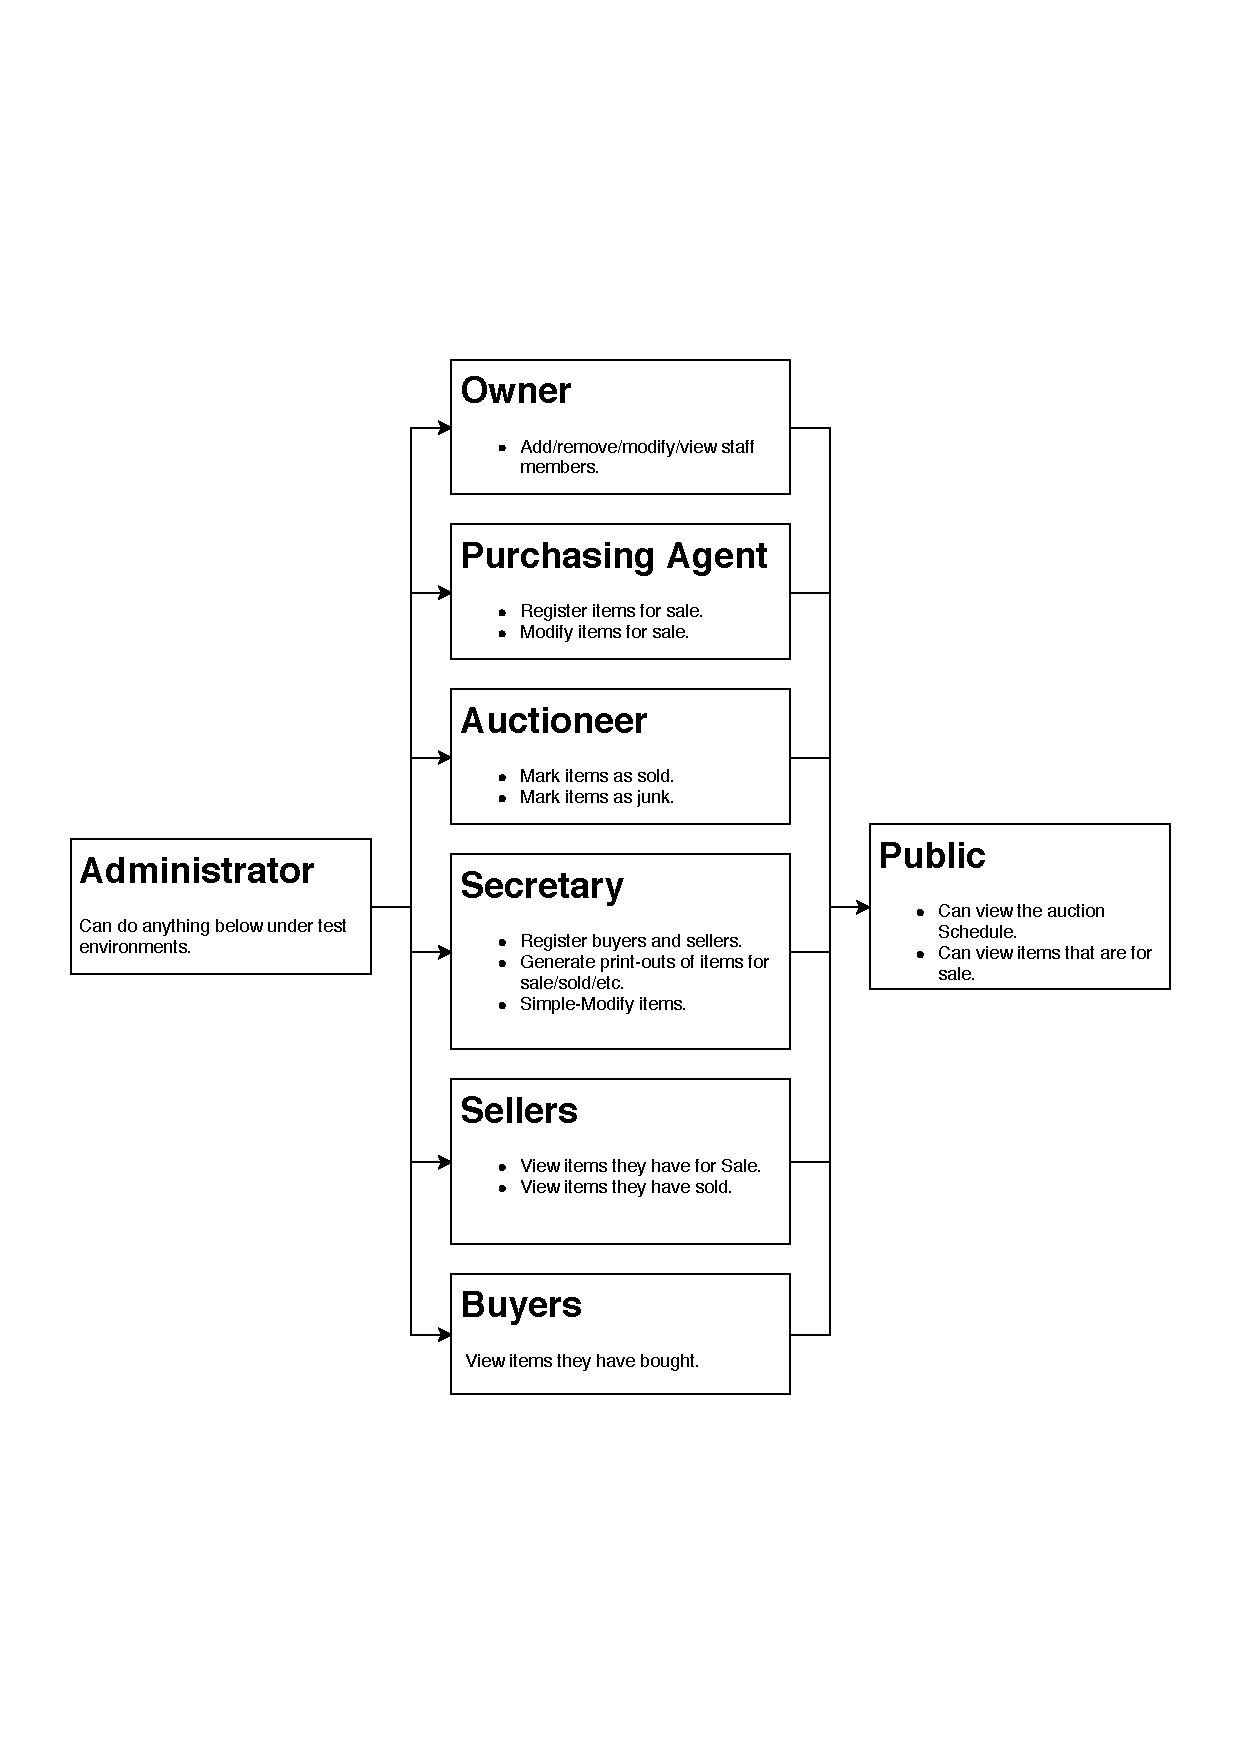
\includegraphics[scale=.75]{power_tree.pdf}
	\caption*{A power tree showing the relations between user groups and permissions. Arrows indicate what permissions are inherited}
\end{figure}

\section*{Use Cases}
% layout and sectioning from Slides week 1, page 25
\subsection*{Create and add an item - Robbin de Groot}
\subsubsection*{Analysis}
\begin{tabular}{@{}l l}
\textbf{Scope}:&The AuctionHouse\textsuperscript{TM} automated administration system\\
\textbf{Level}:&User goal\\
\textbf{Primary Actor}:&Purchasing Agent\\
\textbf{Stakeholders and Interests}:&\begin{tabular}[t]{@{}l}Purchasing Agent: wants to enter parameters easily and quickly\\Seller: wants his goods to be visible to potential buyers\end{tabular}\\
\textbf{Preconditions}:&Purchasing agent is identified and authenticated.\\
\textbf{Postconditions}:&\begin{tabular}[t]{@{}l}The item has been added to the system, or a failure was returned.\\The product has been registered for an upcoming auction.\\The item is (or will become) visible for potential buyers\\and the otherwise authorized.\end{tabular}\\
\textbf{Special requirements}:&A list of categories and a list of future auction dates needs to available in the system\\
\textbf{Frequency of occurence}:&Depedent on the amount of sellers and auctions per month.
\end{tabular}\\\\
\textsl{Main Success Scenario}
\begin{enumerate}[noitemsep]
	\item The user starts the transaction.
	\item The system provides the user with a list of categories to choose from, and a list of future planned aution dates.
	\item The user provides all necessary information and chooses a category for the item, and an auction date. The information to provide is
	\begin{itemize}[noitemsep]
		\item The amount of the item available
		\item The type of item
		\item A description
		\item If the item possesses any antiquarian value
		\item A minimum price decided by the owner
		\item The date when brought in
		\item Name and address of the owner plus identification
		\item Planned auction date
		\item Distinguishing features
	\end{itemize}
	\item The system adds the item with all information to the list
	\item The system returns to the user with a confirmation message or a failure
\end{enumerate}
\textsl{Extensions}
\begin{itemize}[noitemsep]
	\item When a failure is returned, the system database remains unchanged; no item or other information was added.
	\item When not all required information was provided, the system will first ask the user to provide it until all information is provided.
\end{itemize}
\textsl{System Sequence Diagram}
\begin{figure}[H]
	\centering
	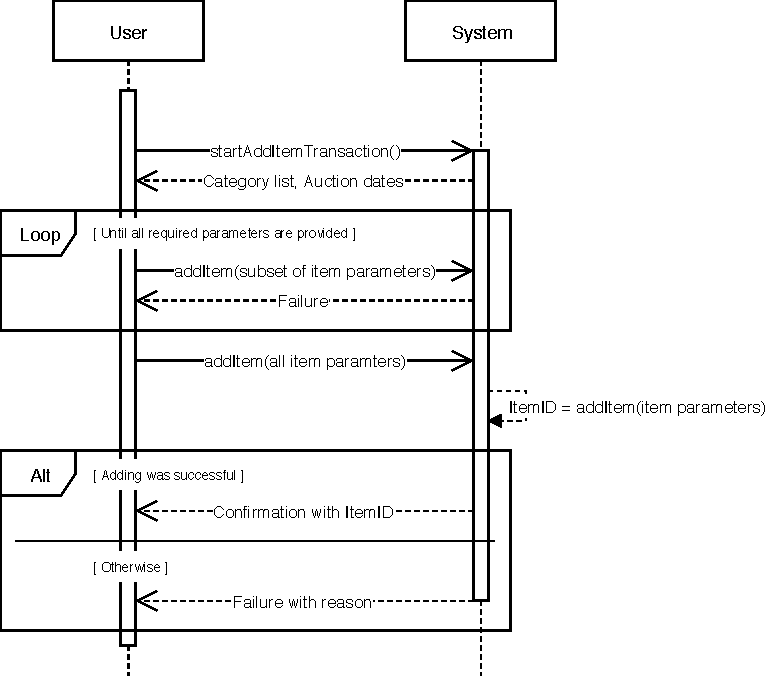
\includegraphics[scale=1]{SD-bb-create.pdf}
	\caption*{Interactions displayed in a System Sequence Diagram in blackbox format}
\end{figure}

\subsubsection*{Design}
\subsection*{Updating - Oliver Strik}
\subsubsection*{Analysis}
\begin{tabular}{@{}l l}
\textbf{Scope}:&The AuctionHouse\textsuperscript{TM} automated administration system\\
\textbf{Level}:&User goal\\
\textbf{Primary Actor}:&Purchasing Agent, Auctioneer, Secretary\\
\textbf{Stakeholders and Interests}:&\begin{tabular}[t]{@{}l}Purchasing Agent, Auctioneer, Secretary: wants to update item parameters quickly and easly.\end{tabular}\\
\textbf{Preconditions}:&Actor is identified and authenticated.\\
\textbf{Postconditions}:&\begin{tabular}[t]{@{}l}The item has been updated on the system, or a failure was returned.\\The updates to the item are (or will become) visible for potential buyers\\and the otherwise authorized.\end{tabular}\\
\textbf{Special requirements}:&\begin{tabular}[t]{@{}l}The current information of an item and a list of future auction dates needs to available\\in the system.\end{tabular}\\
\textbf{Frequency of occurence}:&Frequent\\
\end{tabular}\\\\
\textsl{Main Success Scenario}
\begin{enumerate}[noitemsep]
	\item The user starts the transaction.
	\item The system provides the user with the current information of the item that they are authorised to edit.
	\item The user provides the updated information. The information that can be updated is
	\begin{itemize}[noitemsep]
		\item The amount of the item available
		\item The type of item
		\item A description
		\item If the item possesses any antiquarian value
		\item A minimum price decided by the owner
		\item The date when brought in
		\item Name and address of the owner plus identification
		\item Planned auction date
		\item Distinguishing features
	\end{itemize}
	\item The system updates the item with the given information.
	\item The system returns to the user whether it was successful.
\end{enumerate}
\textsl{Extensions}
\begin{itemize}[noitemsep]
	\item If unsucessful, the system database remains unchanged; no item or other information was added or changed.
\end{itemize}
\textsl{System Sequence Diagram}
\begin{figure}[H]
	\centering
	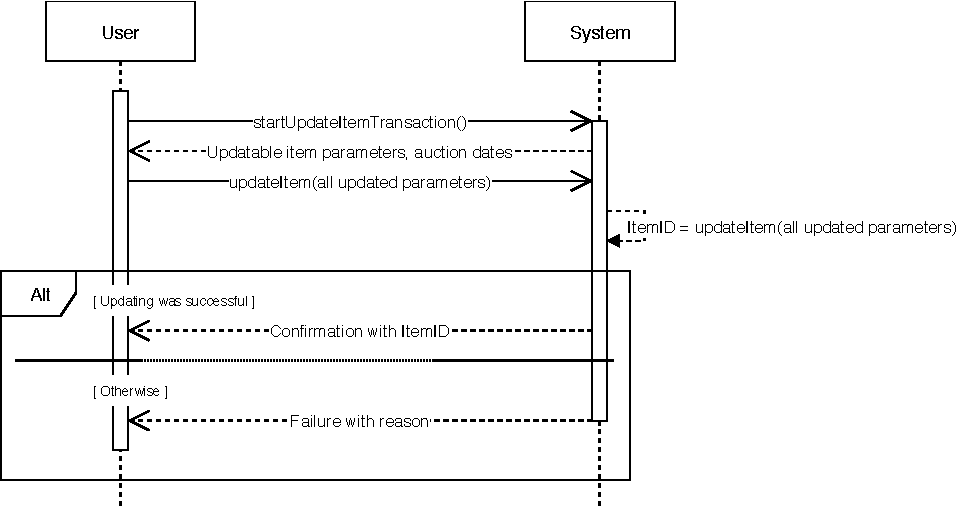
\includegraphics[scale=1]{SD-bb-update.pdf}
	\caption*{Interactions displayed in a System Sequence Diagram in blackbox format}
\end{figure}
\subsubsection*{Design}
\subsection*{Deleting - Nicu Ghidirimischi}
\subsubsection*{Analysis}
\subsubsection*{Design}
\section*{Overall}
\section*{References}
\section*{About Possible Implementation (optional)}

% \begin{tabular}{l|l|c}
% User & Wish & CRUD\\\hline\hline
% \makecell[l]{Private Individuals\\Merchants} & Register Goods & \textbf{C}RUD
% Purchasing Agent & Assess goods for sale & C\textbf{R}U\textbf{D}

% \end{tabular}
\end{document}